\begin{figure*}
  \centering
  \begin{subfigure}[b]{\textwidth}
    \centering
    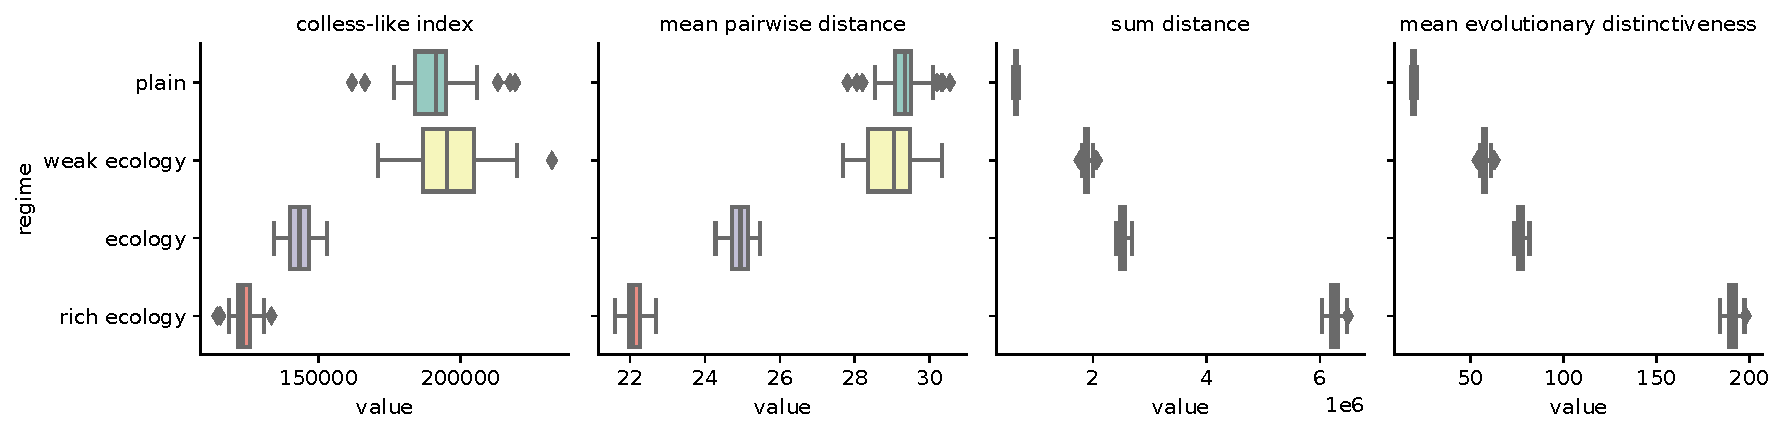
\includegraphics[width=\textwidth]{binder/binder/teeplots/col=phylometric+epoch=0+mut_distn=np.random.standard_normal+nuisance=spatial-structure+viz=boxplot+x=value+y=regime+ext=.pdf}
    \caption{epoch 0 with spatial nuisance}
    \label{fig:perfect-tree-phylometrics-sensitivity-analysis-with-spatial-nuisance:epoch0}
  \end{subfigure}
  \begin{subfigure}[b]{\textwidth}
    \centering
    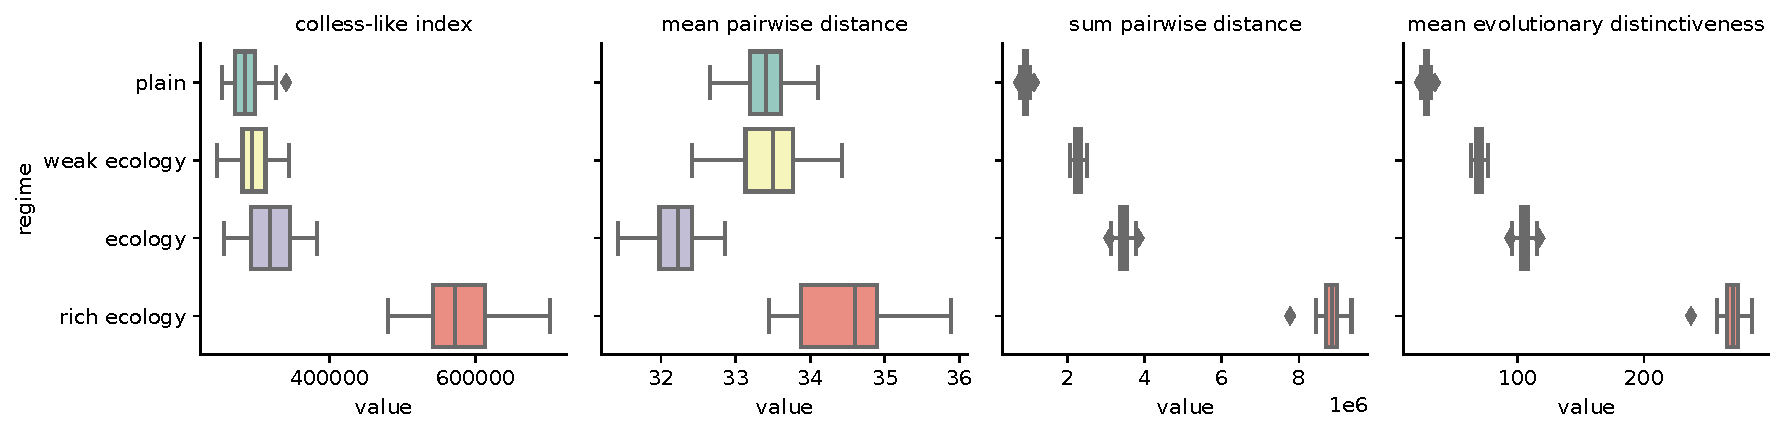
\includegraphics[width=\textwidth]{binder/binder/teeplots/col=phylometric+epoch=2+mut_distn=np.random.standard_normal+nuisance=spatial-structure+viz=boxplot+x=value+y=regime+ext=.pdf}
    \caption{epoch 2 with spatial nuisance}
    \label{fig:perfect-tree-phylometrics-sensitivity-analysis-with-spatial-nuisance:epoch2}
  \end{subfigure}
  \begin{subfigure}[b]{\textwidth}
    \centering
    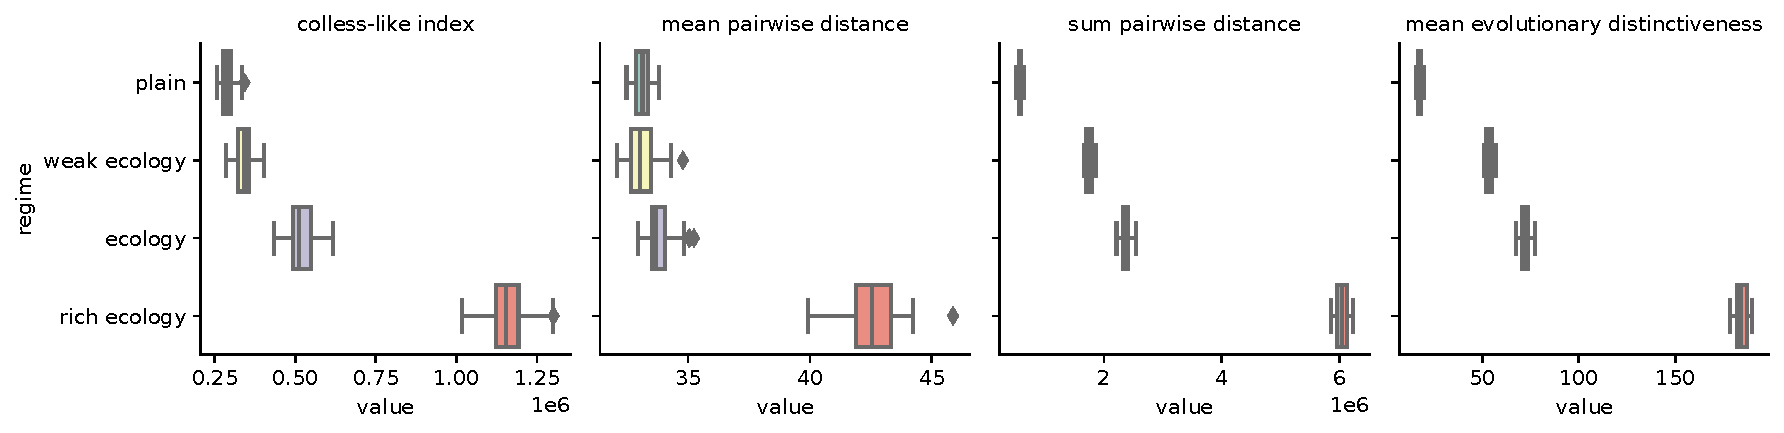
\includegraphics[width=\textwidth]{binder/binder/teeplots/col=phylometric+epoch=0+mut_distn=np.random.exponential+nuisance=spatial-structure+viz=boxplot+x=value+y=regime+ext=.pdf}
    \caption{exponential mutation distribution with spatial nuisance}
    \label{fig:perfect-tree-phylometrics-sensitivity-analysis-with-spatial-nuisance:exponential}
  \end{subfigure}
  \caption{TODO with spatial nuisance}
  \label{fig:perfect-tree-phylometrics-sensitivity-analysis-with-spatial-nuisance}
\end{figure*}
